\documentclass{beamer}

\usepackage[utf8]{inputenc}
\usepackage{amsmath}
\usepackage{graphicx}
\usepackage{pdflscape}
\usepackage{geometry}
\usepackage{xcolor}
\definecolor{darkgreen}{rgb}{0.0, 0.5, 0.0}
\usepackage{bookmark}

\setbeamertemplate{caption}[numbered]
\setbeamercolor{frametitle}{bg=blue, fg=white}

\title{Neural mechanisms in processing of emotion in real and virtual faces}
\subtitle{A functional near-infrared spectroscopy (fNIRS) study}
\author{Dylan Rapanan}
\date{\today}

\begin{document}

\begin{frame}
    \titlepage
\end{frame}

% display C:\Users\super\OneDrive - Ontario Tech University\fNIRS_Emotions\plots\figures\Paradigm.png
\begin{frame}
    \frametitle{Task Paradigm}
    \begin{figure}
        \centering
        \includegraphics[width=0.8\textwidth]{C:/Users/super/OneDrive - Ontario Tech University/fNIRS_Emotions/plots/figures/Paradigm.png}
        \caption{Participants viewed 56 blocks of 8 faces (4 male, 4 female) from two sets:
        real (RADIATE) and virtual (UIBVFED). Each face displayed one of 7
        emotions (anger, disgust, fear, happiness, sadness, surprise, neutral)}
    \end{figure}
\end{frame}

% display C:\Users\super\OneDrive - Ontario Tech University\fNIRS_Emotions\plots\figures\Montage.png
\begin{frame}
    \frametitle{fNIRS Montage}
    \begin{minipage}[t]{0.55\textwidth}
        \vspace{-\baselineskip}
        \includegraphics[width=\textwidth]{C:/Users/super/OneDrive - Ontario Tech University/fNIRS_Emotions/plots/figures/Montage.png}
    \end{minipage}
    % display C:\Users\super\OneDrive - Ontario Tech University\fNIRS_Emotions\plots\figures\Montage legend.png next to the above image
    \begin{minipage}[t]{0.2\textwidth}
        \vspace{-\baselineskip}
        \includegraphics[width=\textwidth]{C:/Users/super/OneDrive - Ontario Tech University/fNIRS_Emotions/plots/figures/Montage legend.png}
    \end{minipage}
    \begin{figure}
        \caption{High density 32x32 fNIRS probe layout with 206 channels. \newline
        fNIRS data recorded using two NIRSport2 systems with sampling rate: 6.105 Hz at wavelengths: 760 $nm$ and 850 $nm$.}
    \end{figure}
\end{frame}

\begin{frame}
    \frametitle{Signal Quality Metrics}
    \begin{itemize}
        \item \textbf{Scalp Coupling Index (SCI):}
        \begin{itemize}
            \item Calculated as the zero-lag cross-correlation between the optical density (OD) signals at two wavelengths. 
            \item A high SCI value ($>$ 0.7) indicates strong synchronization of cardiac pulsations between the two wavelengths, suggesting good optode-scalp contact.
        \end{itemize}
        \item \textbf{Peak Spectral Power (PSP):}
        \begin{itemize}
            \item Measures the amplitude of the most prominent frequency component within a specific range, focusing on the cardiac pulsation.
            \item A higher PSP value ($>$ 0.1) indicates stronger cardiac signal, correlating with better optode-scalp contact.
        \end{itemize}
    \end{itemize}
\end{frame}

% display C:\Users\super\OneDrive - Ontario Tech University\fNIRS_Emotions\plots\signal quality\Percentage of Good Windows.png
\begin{frame}
    \frametitle{Signal Quality by Participant}
    \begin{figure}
        \includegraphics[width=1\textwidth]{C:/Users/super/OneDrive - Ontario Tech University/fNIRS_Emotions/plots/signal quality/Percentage of Good Windows.png}
        \caption{PSP and (SCI) were calculated for 5s sliding windows for each channel for each participant.
        The dotted green line represents the 70\% threshold for good windows.
        }
            \begin{itemize}
                \item If $>$ 70\% of the windows in a channel were good, the channel was deemed good.
                \item If $>$ 70\% of the channels in a participant were good, the participant was deemed good.
                \item 39/87 participants are currently deemed good.
            \end{itemize}
    \end{figure}
\end{frame}

% display C:\Users\super\OneDrive - Ontario Tech University\fNIRS_Emotions\plots\signal quality\Average SCI (Windowed) per Channel\All Participants.png
\begin{frame}
    \frametitle{Signal Quality by Channel}
    \begin{figure}
        \includegraphics[width=1\textwidth]{C:/Users/super/OneDrive - Ontario Tech University/fNIRS_Emotions/plots/signal quality/Average SCI (Windowed) per Channel/All Participants.png}
        \caption{Average SCI for each channel across all participants. The channels are color coded by brain region. The wider the line, the more participants had a SCI value in that range.}
            \begin{itemize}
                \item We can see that the channels towards the back of the head tend to have lower SCI values (this may be because people have lots of hair at the back of their head).
                \item There are a select few channels that have low SCI values across all participants. 
            \end{itemize}
    \end{figure}
\end{frame}

% display C:\Users\super\OneDrive - Ontario Tech University\fNIRS_Emotions\plots\figures\Sample Design Matrix.png
\begin{frame}{General Linear Model (GLM) Analysis}
    \begin{itemize}
        \item \textbf{Purpose:} GLM's are used to understand the relationship between 1+ independent variables and a dependent variable.
        \item \textbf{Design Matrix:}
        \begin{itemize}
            \item It encodes the timing + duration of the conditions. 
            \item Each stimulus is convolved with a Hemodynamic Response Function (HRF) to model the expected brain response. 
            \item This transforms the stimulus onsets into a predictor that mimics the typical shape of the haemodynamic response.
        \end{itemize}
    \end{itemize}
    \begin{figure}
        \includegraphics[width=0.7\textwidth]{C:/Users/super/OneDrive - Ontario Tech University/fNIRS_Emotions/plots/figures/Sample Design Matrix.png}
        \caption{Design matrix (face type) for a single participant (first 150s). Each condition is represented by a different color and represents the onset of a block. The HRF used here is 'spm' (Statistical Parametric Mapping).}
    \end{figure}
\end{frame}

\begin{frame}{General Linear Model (GLM) Analysis}
    \begin{itemize}
        \item \textbf{GLM Estimation:}
        \begin{itemize}
            \item The model fits the observed signal as a linear combination of the predictors in the design matrix:
            \[
            \text{Observed Signal} = \theta_1 \times \text{Predictor}_1 + \cdots + \theta_n \times \text{Predictor}_n + \epsilon
            \]
            \(\theta_1, \theta_2, \ldots, \theta_n\) are the coefficients the model estimates, and \(\epsilon\) is the error term (noise/unexplained variance).
            \item It then applies a fitting algorithm (Ordinary Least Squares) to find the best set of \(\theta\)'s that minimizes the difference between the predicted and actual signals.
            \item The \(\theta\)'s indicate the strength of the brain's response to each experimental condition.
        \end{itemize}
    \end{itemize}
\end{frame}

% display C:\Users\super\OneDrive - Ontario Tech University\fNIRS_Emotions\plots\glm\group_results\results_face_type.png
\begin{frame}{GLM Analysis}
    \begin{itemize}
      \item \textbf{Group-Level Analysis:} $\theta \sim -1 + \text{ROI}:\text{Condition}:\text{Chroma}$
        \begin{itemize}
            \item This mixed effects model estimates separate coefficients ($\theta$'s) for each combination of Region of Interest (ROI), condition, and channel type without a global intercept. 
            \item Group by participant for variability between subjects.
        \end{itemize}
    \end{itemize}
    \begin{figure}
        \includegraphics[width=1\textwidth]{C:/Users/super/OneDrive - Ontario Tech University/fNIRS_Emotions/plots/glm/group_results/results_face_type.png}
        \caption{Swarm plots display $\theta$'s across conditions/ROIs for each channel type. Higher $\theta$ values indicate stronger responses.}
    \end{figure}
\end{frame}

% display C:\Users\super\OneDrive - Ontario Tech University\fNIRS_Emotions\plots\glm\contrasts\differences\Contrast_Real-Virt.png
% display C:\Users\super\OneDrive - Ontario Tech University\fNIRS_Emotions\plots\glm\contrasts\differences\Contrast_Real-Base.png
% display C:\Users\super\OneDrive - Ontario Tech University\fNIRS_Emotions\plots\glm\contrasts\differences\Contrast_Anger-Surprise.png
% display these three side by side
\begin{frame}
    \frametitle{GLM Contrasts}
    \begin{itemize}
        \item \textbf{Contrasts:}
        \begin{itemize}
            \item Contrasts between pairs of conditions (i.e. \texttt{Joy - Fear}) are defined by subtracting corresponding regressors. 
            \item This highlights the differences in haemodynamic responses under the combinations of conditions.
        \end{itemize}
    \end{itemize}
    \begin{minipage}[t]{0.3\textwidth}
        \vspace{-\baselineskip}
        \includegraphics[width=\textwidth]{C:/Users/super/OneDrive - Ontario Tech University/fNIRS_Emotions/plots/glm/contrasts/differences/Contrast_Real-Virt.png}
        \end{minipage}
        \begin{minipage}[t]{0.3\textwidth}
        \vspace{-\baselineskip}
        \includegraphics[width=\textwidth]{C:/Users/super/OneDrive - Ontario Tech University/fNIRS_Emotions/plots/glm/contrasts/differences/Contrast_Real-Base.png}
        \end{minipage}
        \begin{minipage}[t]{0.3\textwidth}
        \vspace{-\baselineskip}
        \includegraphics[width=\textwidth]{C:/Users/super/OneDrive - Ontario Tech University/fNIRS_Emotions/plots/glm/contrasts/differences/Contrast_Anger-Surprise.png}
        \end{minipage}  \begin{figure}
        \caption{Contrast maps (Hbo) for Real vs. Virtual (left), Real vs. Baseline (middle), and Anger vs. Surprise (right).}
        \begin{itemize}
            \item Only channels with \(P < |z|\) less than 0.05 are displayed, indicating a significant difference in Hbo.
        \end{itemize}
    \end{figure}
\end{frame}

% display C:\Users\super\OneDrive - Ontario Tech University\fNIRS_Emotions\plots\erp\erp_conditions\Real.png
\begin{frame}
    \frametitle{Event Related Potentials (ERPs)}
    \begin{figure}
        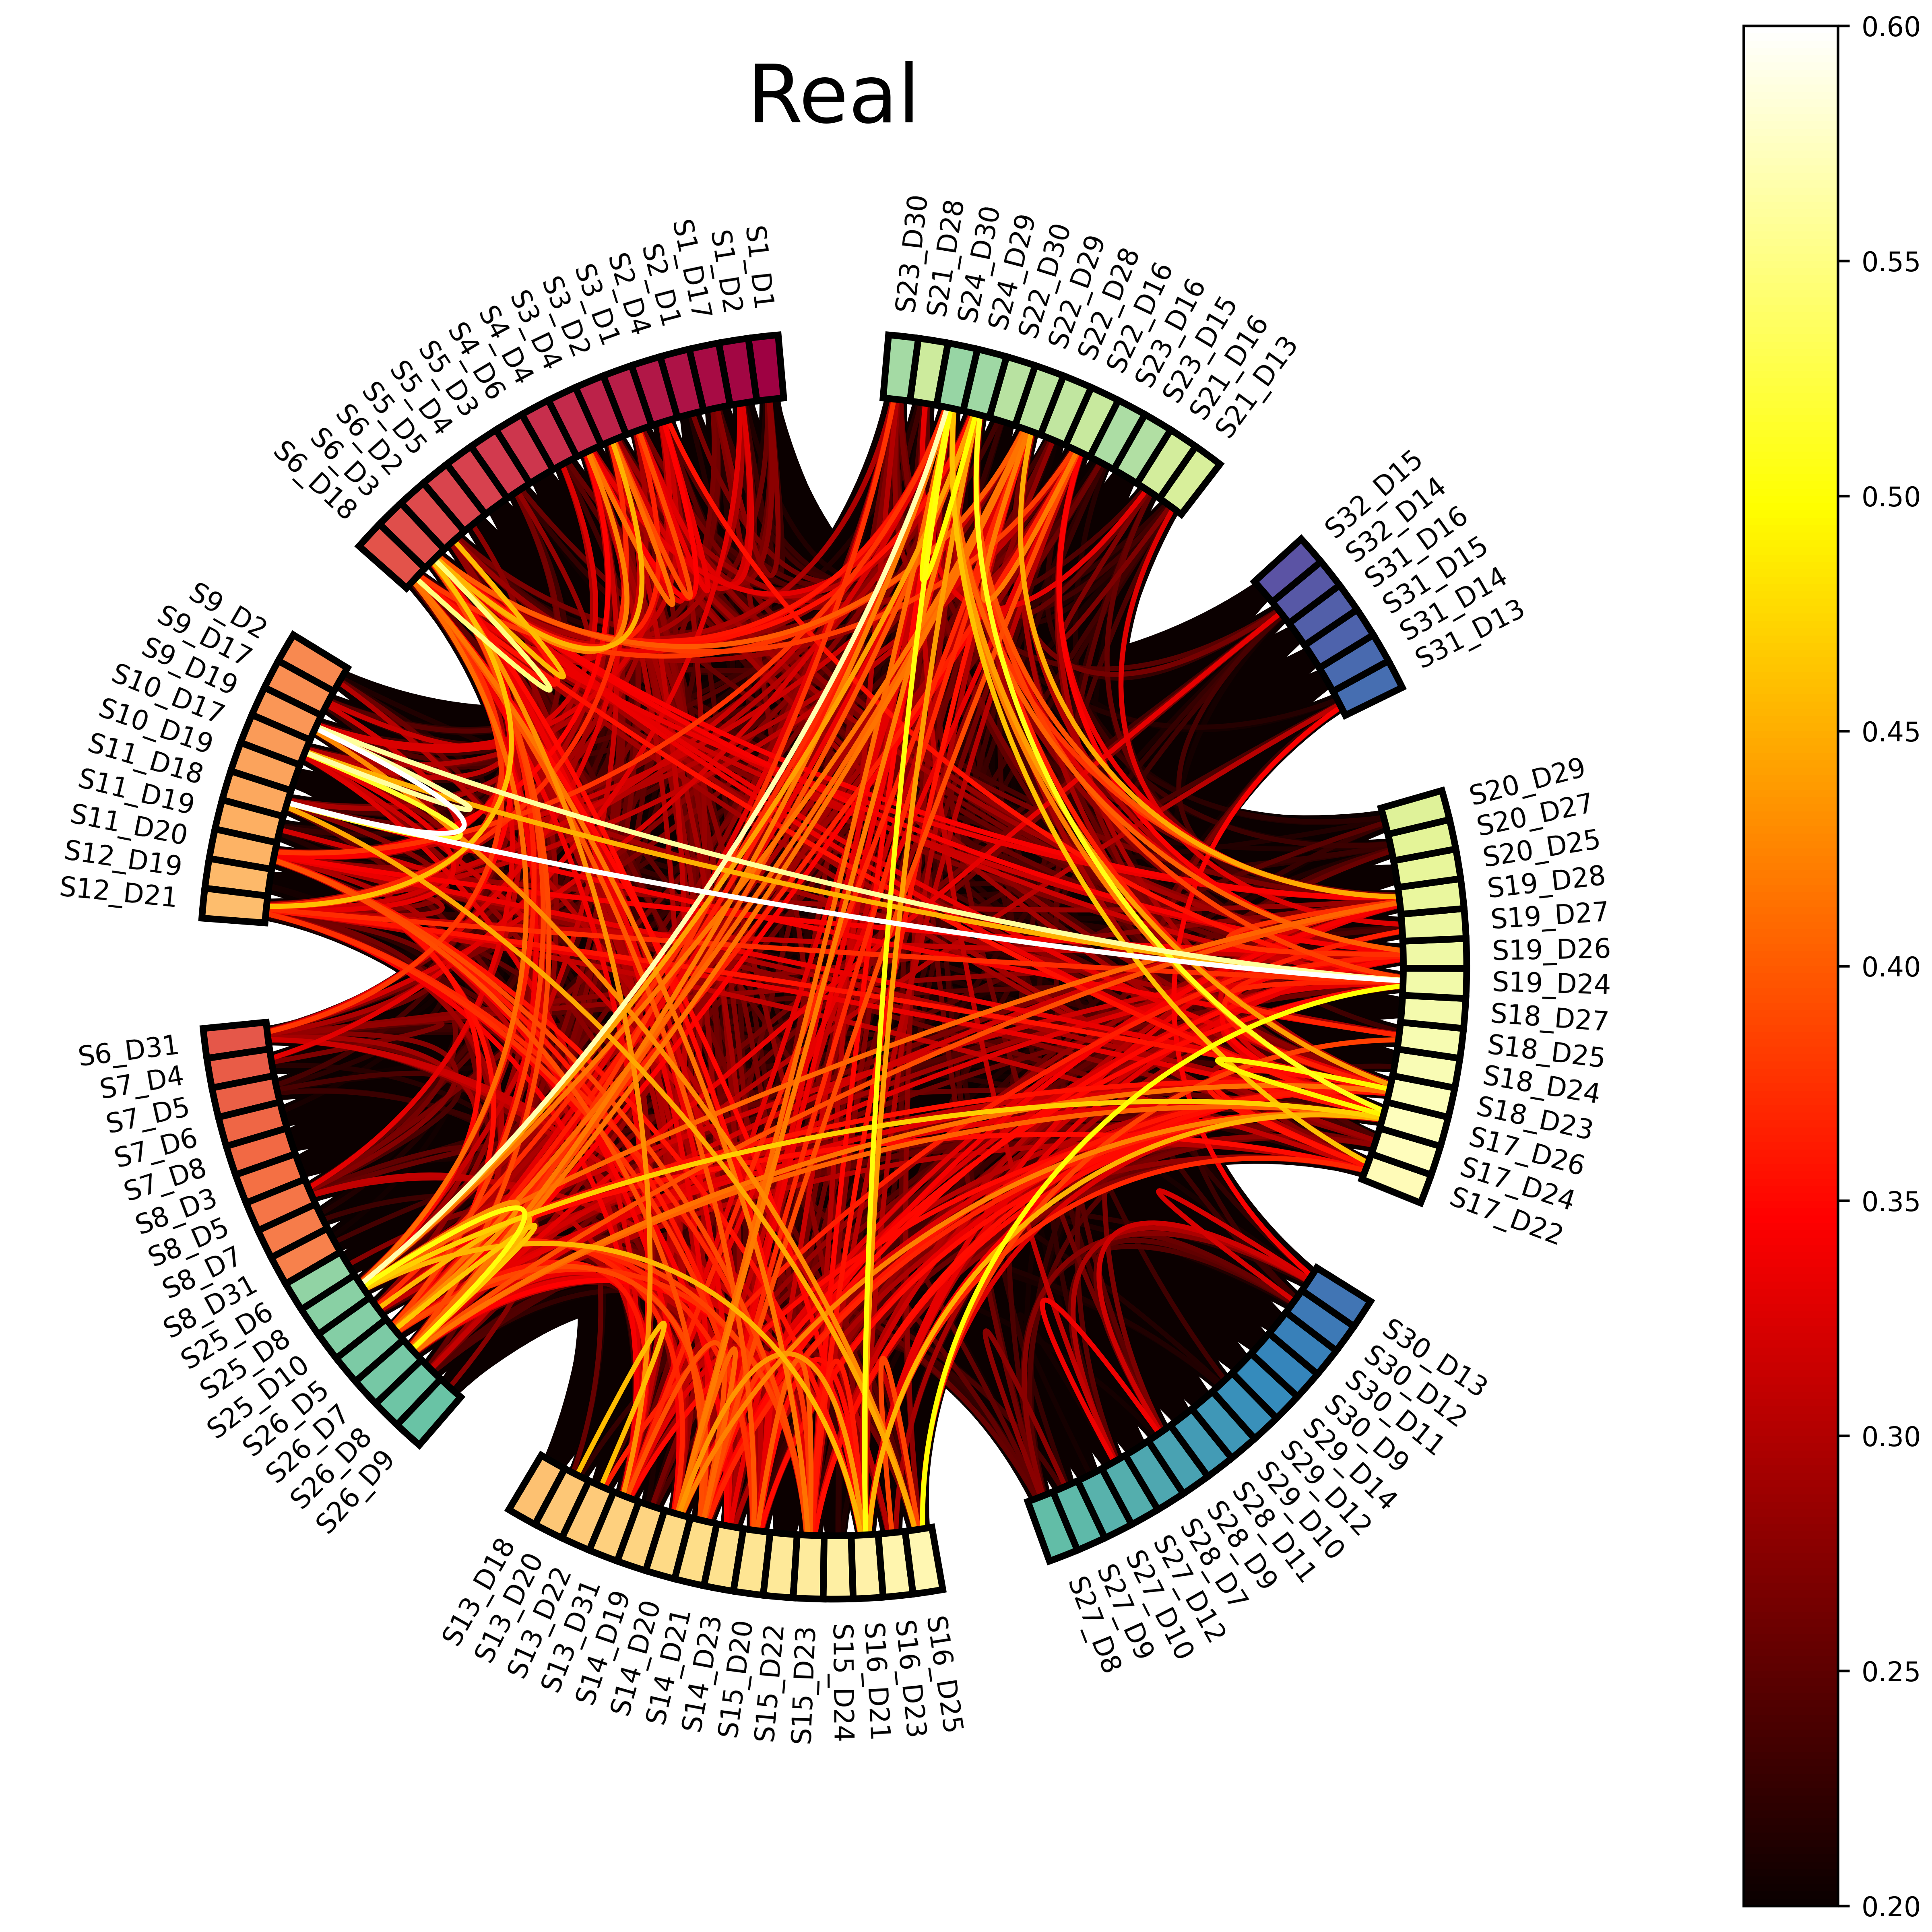
\includegraphics[width=1\textwidth]{C:/Users/super/OneDrive - Ontario Tech University/fNIRS_Emotions/plots/erp/erp_conditions/Real.png}
        \caption{ERP for real face epochs across all channels. The x-axis represents time in seconds ($s$) and the y-axis represents the $\Delta$Hbo/Hbr/Hbt in micromolars ($\mu M$).}
        \begin{itemize}
            \item The shaded region is the standard error of the mean: $\frac{\sigma}{\sqrt{n}}$. 
        \end{itemize}
    \end{figure}
\end{frame}

% display C:\Users\super\OneDrive - Ontario Tech University\fNIRS_Emotions\plots\erp\erp_differences\Fear_Sadness.png
\begin{frame}
    \frametitle{ERP Differences}
    \begin{figure}
        \includegraphics[width=1\textwidth, trim=0 1290 0 0, clip]{C:/Users/super/OneDrive - Ontario Tech University/fNIRS_Emotions/plots/erp/erp_differences/Fear_Sadness.png}
        \caption{ERP difference in Hbo between fear and sadness for Left/Right frontal regions. }
    \end{figure}
\end{frame}

% display C:\Users\super\OneDrive - Ontario Tech University\fNIRS_Emotions\plots\erp\erp_differences\Fear_Sadness.png
\begin{frame}
    \frametitle{ERP Differences}
    \begin{figure}
        \includegraphics[width=1\textwidth, trim=0 0 0 1275, clip]{C:/Users/super/OneDrive - Ontario Tech University/fNIRS_Emotions/plots/erp/erp_differences/Fear_Sadness.png}
        \caption{ERP difference in Hbo between fear and sadness for Left/Right occipital regions. }
    \end{figure}
\end{frame}

\begin{frame}
    \frametitle{Connectivity Analysis Methodology}
    \begin{itemize}
        \item \textbf{Connectivity Analysis:} We analyze the relationship between channels to understand how different regions of the brain communicate.
        \item \textbf{Parameters:}
            \begin{itemize}
                \item \textcolor{darkgreen}{\# Coherence as the connectivity metric:}
                \begin{itemize}
                    \item \texttt{method = "coh"}
                \end{itemize}
                \item \textcolor{darkgreen}{\# CWT with Morlet wavelets for time-frequency analysis:}
                \begin{itemize}
                    \item \texttt{con\_mode = "cwt\_morlet"}
                \end{itemize}
                \item \textcolor{darkgreen}{\# Analyze frequencies ranging from 0.01 Hz to 0.5 Hz:}
                \begin{itemize}
                    \item \texttt{cwt\_freqs = np.linspace(0.01, 0.5, 10)}
                \end{itemize}
                \item \textcolor{darkgreen}{\# Use 1 cycle per frequency for wavelet transformation:}
                \begin{itemize}
                    \item \texttt{cwt\_n\_cycles = 1}
                \end{itemize}
                \item \textcolor{darkgreen}{\# Average connectivity matrices across frequencies:}
                \begin{itemize}
                    \item \texttt{faverage = True}
                \end{itemize}
            \end{itemize}
    \end{itemize}
\end{frame}

% display C:\Users\super\OneDrive - Ontario Tech University\fNIRS_Emotions\plots\connectivity\heatmaps\individual\face_type_Virt_cons\con_31.png
% display C:\Users\super\OneDrive - Ontario Tech University\fNIRS_Emotions\plots\connectivity\heatmaps\conditions\face_type_Virt_con.png
% display these two side by side
\begin{frame}
    \frametitle{Connectivity Analysis}
    \begin{minipage}[t]{0.49\textwidth}
        \vspace{-\baselineskip}
        \includegraphics[width=\textwidth, trim=150 150 140 150, clip]{C:/Users/super/OneDrive - Ontario Tech University/fNIRS_Emotions/plots/spectral_connectivity_time/heatmaps/individual/face_type_Virt_cons/con_31.png}
        \end{minipage}
        \begin{minipage}[t]{0.49\textwidth}
        \vspace{-\baselineskip}
        \includegraphics[width=\textwidth, trim=150 150 140 150, clip]{C:/Users/super/OneDrive - Ontario Tech University/fNIRS_Emotions/plots/spectral_connectivity_time/heatmaps/conditions/face_type_Virt_con.png}
    \end{minipage}
    \begin{figure}
        \caption{Virtual face connectivity heatmaps for a single participant (left) and the average across all participants (right).
        The x-axis/y-axis represent the channel. A brighter color \(\implies\) higher connectivity strength.}
        \begin{itemize}
            \item The averaged heatmap has a more washed out distribution.
        \end{itemize}
    \end{figure}
\end{frame}

% display C:\Users\super\OneDrive - Ontario Tech University\fNIRS_Emotions\plots\connectivity\chord_plots\conditions\emotion_Sadness_con.png
% display C:\Users\super\OneDrive - Ontario Tech University\fNIRS_Emotions\plots\connectivity\chord_plots\conditions\face_type_Base_con.png
% display these two side by side
\begin{frame}
    \frametitle{Connectivity Chord Plots}
    \begin{minipage}[t]{0.45\textwidth}
        \vspace{-\baselineskip}
        \includegraphics[width=\textwidth]{C:/Users/super/OneDrive - Ontario Tech University/fNIRS_Emotions/plots/spectral_connectivity_time/chord_plots/conditions/emotion_Sadness_con.png}
    \end{minipage}
    \begin{minipage}[t]{0.45\textwidth}
        \vspace{-\baselineskip}
        \includegraphics[width=\textwidth]{C:/Users/super/OneDrive - Ontario Tech University/fNIRS_Emotions/plots/spectral_connectivity_time/chord_plots/conditions/face_type_Base_con.png}
    \end{minipage}
    \begin{figure}
        \caption{Chord plot of connectivity between channels for sadness (left) and baseline (right) conditions. Brighter lines represent higher connectivity strength.}
        \begin{itemize}
            \item Connections across the middle of the plot indicate connectivity across far apart regions of the brain.
        \end{itemize}
    \end{figure}
\end{frame}

% display C:\Users\super\OneDrive - Ontario Tech University\fNIRS_Emotions\plots\connectivity\chord_plots\group_level_t_tests\face_type_Real_Virt_p_values.png
% display C:\Users\super\OneDrive - Ontario Tech University\fNIRS_Emotions\plots\connectivity\chord_plots\group_level_t_tests_neutral\emotion_Joy_Neutral_p_values.png
% display these two side by side
\begin{frame}
    \frametitle{Connectivity Group Level T-Tests Chord Plots}
    \begin{minipage}[t]{0.45\textwidth}
        \vspace{-\baselineskip}
        \includegraphics[width=\textwidth]{C:/Users/super/OneDrive - Ontario Tech University/fNIRS_Emotions/plots/spectral_connectivity_time/chord_plots/group_level_t_tests_roi/face_type_Real_Virt.png}
    \end{minipage}
    \begin{minipage}[t]{0.45\textwidth}
        \vspace{-\baselineskip}
        \includegraphics[width=\textwidth]{C:/Users/super/OneDrive - Ontario Tech University/fNIRS_Emotions/plots/spectral_connectivity_time/chord_plots/group_level_t_tests_roi/emotion_Joy_Neutral.png}
    \end{minipage}
    \begin{figure}
        \caption{Paired t-tests were conducted for each unique pair of conditions (i.e. Real vs. Virtual (left) and Joy vs. Neutral (right)).
        $p$-values were computed for each channel pair across participants. }
        \begin{itemize}
            \item False Discovery Rate (FDR) correction was applied, which controls the expected proportion of false positives among all significant results when conducting multiple hypothesis tests.
        \end{itemize}
    \end{figure}
\end{frame}

\begin{frame}{Decoding Analysis Methodology}
    \begin{itemize}
        \item \textbf{Data Preprocessing:}
        \begin{itemize}
            \item \textbf{Scaler:} Scales each channel to zero mean and unit variance.
            \item \textbf{Vectorizer:} Flattens data into a 2D feature matrix.
            \item \textbf{Model:} Pick the classifier (e.g., \texttt{RandomForestClassifier}). 
        \end{itemize}
        \item \textbf{Cross-Validation:} 
        \begin{itemize}
            \item We perform 5-fold cross-validation, where data is split into 5 folds, preserving the class distribution (stratified splitting).
        \end{itemize}
        \item \textbf{Scoring:}
        \begin{itemize}
            \item \textbf{ROC-AUC Score:} A single metric that quantifies a model's ability to distinguish between classes by calculating the area under the ROC curve, where 1.0 indicates perfect discrimination and 0.5 represents random guessing.
            \item Each fold is evaluated using the ROC-AUC score with the one-vs-rest (OVR) approach for multiclass evaluation.
        \end{itemize}
        \item \textbf{Aggregation:}
        \begin{itemize}
            \item Mean of the scores across folds are computed for each participant, providing a robust estimate of model performance and its variability.
        \end{itemize}    
    \end{itemize}
\end{frame}

% display C:\Users\super\OneDrive - Ontario Tech University\fNIRS_Emotions\plots\models\model_scores.png
\begin{frame}
    \frametitle{Decoding Analysis Results}
    \begin{figure}
        \includegraphics[width=1\textwidth]{C:/Users/super/OneDrive - Ontario Tech University/fNIRS_Emotions/plots/models/raw_scores.png}
        \caption{Spatio-temporal classification performance of multiple machine learning models across conditions. For each model, recordings were preprocessed via scaling and vectorization. The average ROC-AUC scores were computed using five-fold cross-validation over all recordings. }
        \begin{itemize}
            \item The \texttt{RandomForestClassifier} model performed the best in identifying the face type, while the \texttt{LGBMClassifier} model performed the best in identifying the emotion.
        \end{itemize}
    \end{figure}
\end{frame}

\begin{frame}
    test
\end{frame}

\end{document}